\chapter{Base Teórica}
\epigraph{\textit{To see the world in a grain of sand, and to see heaven in a wild flower, hold infinity in the palm of your hands, and eternity in an hour.}}{-William Blake}
Este capítulo introduz os conceitos essenciais necessários para o entendimento deste trabalho. Na primeira parte são apresentadas as bases de confiabilidade, robustez e falhas em sistemas. A segunda parte apresenta detalhes sobre os efeitos físicos que surgem em trasistores CMOS que levam ao envelhecimento dos mesmos, os modelos empregados para estimar tais efeitos.

Em adição, é apresentado o estado da arte em confiabilidade de circuitos integrados e uma introdução aos atuais simuladores que auxiliam nesta tarefa e de que forma eles atuam.
\section{Confiabilidade}
A confiabilidade de um sistema é definida como a ``probabilidade de que uma porção de sistema irá durar por pelo menos um tempo previamente especificado sob a ação de condições experimentais especificadas'' \cite{Maricau2013}.
Dado que é esperado que um sistema obedeça suas condições de operação especificadas por um tempo mínimo sem que apresente problemas ou se mostre confiável, podemos analisar, prever e informar a sistemas supervisores quais condições levariam a interrupções no funcionamento adequado do sistema observado.
Para compor esta análise, é utilizado um conjunto de métricas para eventos de falha e recuperação de falhas para um sistema, quais sejam \cite{Sorin2009}\cite{Seymour1993}:
\begin{enumerate} 
\item \textbf{MTTF - Mean time to failure:} é o tempo médio que leva até que um sistema falhe;\item \textbf{MTTR – Mean time to repair:} é o tempo médio que o sistema necessita para retornar à operação normal;\item \textbf{MTBF – Mean time between failures:} é o tempo médio que o sistema leva entre falhas. Neste caso é levado em consideração o tempo de recuperação, anteriormente definido;\item \textbf{FIT – Failures in time:} é a razão de falhas que acontecem em um sistema em 1 bilhão de horas.
\end{enumerate}
Já para a definição de uma falha é preciso considerar as seguintes definições \cite{Sorin2009}:
\begin{enumerate}
\item \textbf{Faltas:} considerada uma falha física, tais como condutores quebrados, transistores com portas danificadas, resistores queimados;\item \textbf{Erro:} A falta acima definida pode se manifestar em um erro, que é a troca ou incorreta representação da informação que o meio físico deveria permitir, como bits trocados dentro de uma memória;\item \textbf{Falha:} O erro por sua vez pode se manifestar visivelmente como um comportamento indesejado, apresentando-se como operações errôneas, travamentos ou até indisponibilidade de um sistema, incorrendo em uma falha.
\end{enumerate}
A disponibilidade de um sistema é uma função de MTBF e MTTF (ou MTTF e MTTR), podendo ser definida pela equação \ref{eq:Disponibilidade} e a relação entre estes é retratada na Figura \ref{figure:grafico_MTTF_MTBF}.

\begin{equation} \label{eq:Disponibilidade}
Disponibilidade = \frac{MTTF}{MTBF}= \frac{MTTF}{MTTF + MTTR}
\end{equation}

\begin{figure}[H]
\center
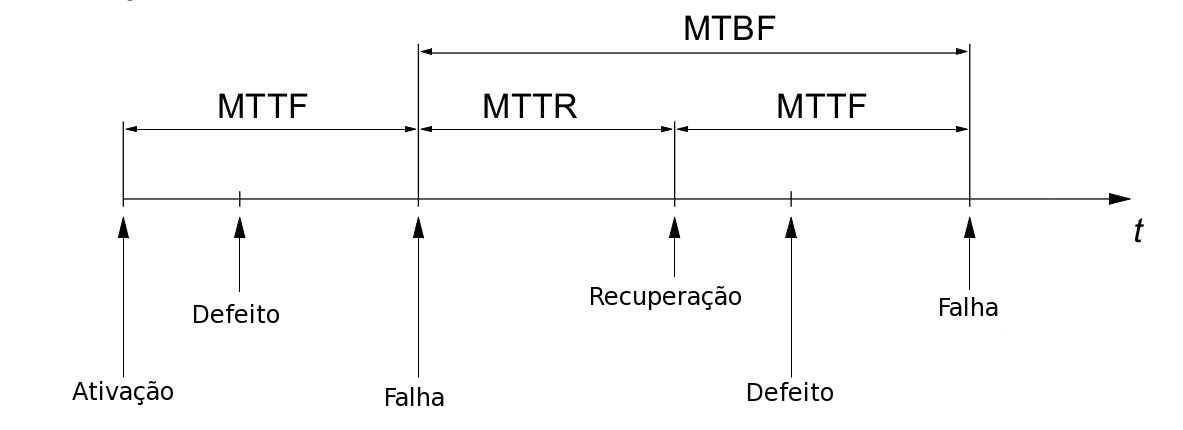
\includegraphics[width=1\textwidth]{images/grafico_mttf_mtbf}
\caption{Relação entre as falhas, defeitos, tempos médios de falha, tempos médios de recuperação e tempo médio entre falhas.}
\label{figure:grafico_MTTF_MTBF}
\end{figure}
Ao ser definida a probabilidade de um sistema operar conforme planejado até um instante de tempo $t$, está sendo definido o que se compreende por \textit{Confiabilidade}. Desta forma, a confiabilidade $R(t)$ de um sistema é normalmente descrita através de um expressão probabilística. Esta por sua vez considera que, para o período $t$ anteriormente mencionado, existe uma taxa de falha $\lambda$ que representa a probabilidade de falha deste sistema para um período $t$ \cite{Calabro1962}.

Na maioria dos casos, uma taxa de falha $\lambda$ constante é assumida \cite{Koren2007}, permitindo que a confiabilidade $R(t)$ seja expressada por uma função exponencial, explicitada na equação \ref{eq:Confiabilidade}.
\begin{equation} \label{eq:Confiabilidade}
R(t) = \textit{e}^{-\lambda t}
\end{equation}
Em concordância com definição de MTTF apresentada anteriormente, a mesma pode ser equacionada conforme mostrada na equação \ref{eq:MTTF}
\begin{equation} \label{eq:MTTF}
MTTF = \int_{0}^{\infty} R(t)dt = \frac{1}{\lambda}
\end{equation}

Para este trabalho o MTTF será empregado como a relação entre um acréscimo no atraso do circuito em uma saída especificada a priori, o acréscimo máximo permitido e o tempo de observação de envelhecimento do dispositivo. É importante salientar que  será abordada a falha $\lambda$ após o período de mortalidade infantil.
\subsection{Confiabilidade em Engenharia}
\label{subsection_Conf_Eng}
A confiabilidade em engenharia estabeleceu-se como um ramo de pesquisa nos tempos modernos, sendo o termo ``confiabilidade'' usado extensivamente pelo público em geral e pela comunidade técnica como sendo a capacidade de um sistema ou componente de operar normalmente sobre certas condições \cite{Maricau2013}. A base para a confiabilidade é a teoria probabilística e estatística, que permitiram o avanço deste campo de estudo tal como é conhecido atualmente. A partir daí, e com o advento da produção em massa de bens de consumo, o estudo da confiabilidade de sistemas se tornou essencial em projetos de engenharia, como foi o caso da (não)confiabilidade de tubos de vácuo \cite{Maricau2013}\cite{Saleh2006}.

Esta preocupação vital perdura até hoje, incluindo sistemas elétricos e eletrônicos de diferentes requisitos, e de forma pervasiva encontra-se em diferentes campos de estudo, tais como: sistemas de potência (modelagem baseada em agentes ou métodos clássicos) \cite{Endrenyi1979}\cite{Schlapfer}, rádio frequência \cite{Stephens2009}\cite{Larcher2006}, tempo de vida restante para transformadores de potência \cite{Osorio}–\cite{Jirutitijaroen2004}, sistemas de supervisão  e intervenção de estados clínicos \cite{LIMOUSIN1997}\cite{Arain2012}).

Os métodos e técnicas utilizadas são desenvolvidos, adaptados e/ou expandidos para esses diversos campos de pesquisa levando em consideração suas particularidades e quais fenômenos contribuem para o surgimento de falhas. Apesar destas particularidades, tais metodologias podem ser estudas em um âmbito mais generalista, sem prejuízo ao estudo de um problema específico \cite{Nelson2004}.

A confiabilidade de circuitos integrados tornou-se essencial para a indústria de CI's, sendo considerada um dos maiores problemas a ser enfrentado em curto prazo, como definido no ``The international technology roadmap for semiconductors''\cite{Hoefflinger2011}, explicitando efeitos como \textit{Time Dependent Dielectric Breakdown, Bias Temperature Instability} e \textit{Hot-Carrier Injection}.

\subsection{Técnicas de confiabilidade e robustez}
\label{subsection_Conf_tecnicas}
Diversas técnicas tem sido desenvolvidas e propostas para mitigar a redução de confiabilidade e robustez de sistemas. Tais técnicas podem abordar o problema diretamente na camada de \textit{hardware} ou de \textit{software}. Em adição, as abordagens pode ser divididas em dois grandes grupos \cite{Siewiorek1992}:
\begin{enumerate} 
\item \textbf{Intolerante à falhas:} Também conhecida como \textit{Prevenção de Falhas}, esta abordagem é considerada conservativa. A premissa neste caso é de que a redução da probabilidade de falha pode ser obtida através da utilização de dispositivos especialmente desenvolvidos para tal intento e/ou da utilização de métodos que propõe prolongar o tempo de vida do sistema;\item \textbf{Tolerante à falhas:} Já nesta abordagem as falhas são toleráveis pelo sistema. Estas técnicas se utilizam de redundâncias para, ou prover tempo extra para que o sistema volte à sua operação normal, ou garantir um caminho extra que, não submetido a uma falha, propague corretamente a informação desejada. 
\end{enumerate}

A seção \ref{subsubsection_tecnicas_hardware} irá sumarizar as propostas de algumas técnicas a nível de \textit{hardware} (\textit{i.e.} nível físico). Este trabalho apresentará posteriormente uma solução intolerante à falhas. É importante salientar que tais técnicas não são, necessariamente, mutuamente exclusivas.

\subsubsection{Técnicas em hardware}
\label{subsubsection_tecnicas_hardware}

De forma geral, as técnicas a nível físico podem ser distinguidas por \cite{Siewiorek1992}:
\begin{enumerate} 
\item \textbf{Modificação das condições ambientais:} engloba um conjunto de medidas que tendem a melhorar as condições ambientais de operação de um sistema, seja através da redução de efeitos degradantes de temperatura, dissipação de calor, radiação, entre outros;
\item \textbf{Melhoria de qualidade:} Neste caso é proposto a utilização de materiais com propriedades superiores ao já normalmente utilizados ou a melhoria da qualidade do processo de fabricação dos componentes que compõe o sistema;
\item \textbf{Duplicação:} é considerada uma técnica relativamente simples para detecção de falhas. Como o próprio nome indica, há uma duplicação de componentes e, havendo a falha em um destes, é feita uma comparação da informação. Uma diferença indica que uma falha ocorreu;
\item \textbf{Códigos para detecção de erros:} para estes casos, é averiguado qual conjunto de informações, de todas as possíveis em um sistema, realmente representa uma informação válida. Isso significa que para um conjunto de bits, por exemplo, apenas uma determinada combinação deles é esperada. A partir daí, uma comparação é realizada para determinar a validade dos dados. Aguns exemplos básicos desta técnica são os bits de paridade, códigos de Hamming e os \textit{checksums};
\item \textbf{Reconfiguração:} neste caso, após detectado o erro ou falha, o sistema altera parcialmente sua estrutura ou comportamento. Isso significa que ele pode combinar as técnicas anteriores, podendo rotear o caminho percorrido pela informação desejada para uma duplicata dos componentes que estão falhos, alterar o instante de sincronização das informações na saída ou até mesmo simplesmente desligar uma porção do sistema, fazendo com que ele opere de forma degradada.
\end{enumerate}


\subsection{Confiabilidade em circuitos integrados}
\label{subsection_Conf_CI}
Na década de 70, os problemas mais comuns de falha de dispositivos estavam relacionados à problemas de empacotamento e montagem (\textit{e.g.,} corros\~{a}o, conexão de fios e contaminação iônica). Somente após o advento de dispositivos integrados menores, efeitos como \textit{Hot Carrier Injection} se tornaram mais preocupantes, uma vez que começaram a afetar o desempenho destes dispositivos.

Encarados inicialmente como de f\'{a}cil prediç\~{a}o (\textit{i.e.,} determinísticos), tais efeitos passaram a ser considerados estocásticos e o primeiro deles a apresentar este comportamento foi o \textit{Time-Dependent Dielectric Breakdown} \cite{Solomon1977}. Estas mudanças surgiram \`{a} medida que a reduç\~{a}o do \'{o}xido do diel\'{e}trico se intensificou, atingindo a escala atômica. Com a continuada redução do tamanho dos dispositivos, entrando então na escala nanométrica, erros estocásticos e variações em nível atômico tornaram-se cada vez mais aparentes.

Variaç\~{o}es no processo de fabricaç\~{a}o surgem, introduzindo variabilidade nos dispositivos, e aumentando os desafios para projetistas de circuitos integrados.
Para este trabalho é importante compreendermos os fenômenos básicos através dos quais cargas ficam presas em determinadas regiões do transistor e como se relacionam com os mecanismos de envelhecimento que serão descritos em seguida. Tendo isto em mente, podemos então dividir os tipos de cargas nas seguintes categorias \cite{Leblebici1993}:
\begin{enumerate}
\item\textbf{Fixas no óxido}: proveniente de defeitos estruturais na camada de óxido que surgem durante processos de oxidação térmica, são encontradas próximas a interface $Si-SiO_2$. Esta região é normalmente descrita por $Si-SiO_x$, sendo uma representação intermediária entre o substrato e óxido. Assim sendo, são independentes das condições de operação do transistor;\item\textbf{Íons móveis no óxido}: são associados às impurezas no próprio óxido decorrentes dos processos de fabricação da estrutura \cite{Bentarzi2011};\item\textbf{Presas no óxido}: juntamente com as cargas presas na interface, tem um importante papel na degradação gradual das características do óxido. Estas cargas possuem energia cinética o suficiente para serem injetadas após vencerem a barreira de potencial da região entre o silício e óxido;\item\textbf{Presas na interface}: semelhantemente, estas cargas possuem uma energia cinética alta o suficiente para vencer a barreira de potencial porém não adentram o óxido, mantendo-se portanto na região interfacial entre o silício e óxido.
\begin{figure}[H]
\center
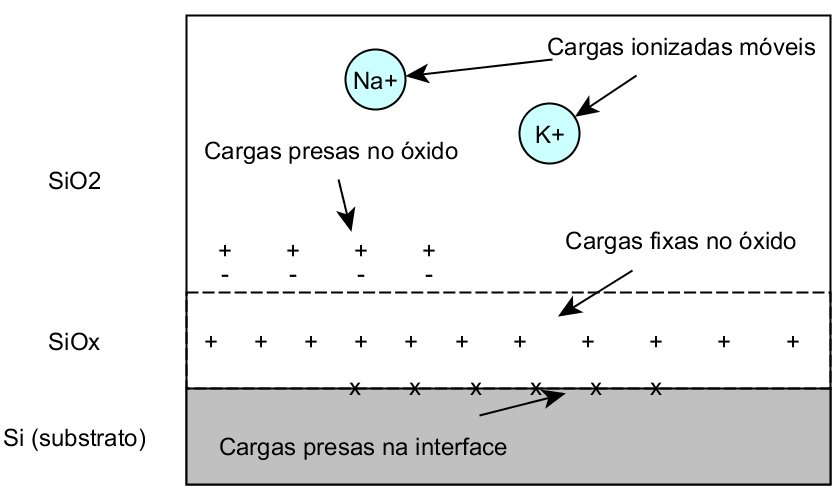
\includegraphics[width=0.5\textwidth]{images/armadilhas_interfaciais}
\caption{Tipos de cargas associadas a um estrutura $Si-SiO_2$.}
\label{figure:armadilhas_interfaciais}
\end{figure}
\end{enumerate}
Diversos modelos atômicos foram propostos para descrever as armadilhas que capturam elétrons e lacunas. A maioria destas armadilhas são usualmente ligações incompletas, como mostradas na figura \ref{figure:modelos_armadilhas}:
\begin{figure}[H]
\center
\subfloat[Interface sem imperfeições\label{figure:interface_perfeita}]{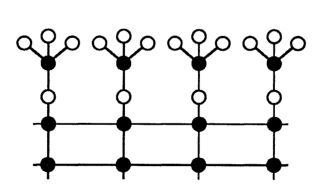
\includegraphics[width=0.4\textwidth]{images/interface_perfeita}}
\hfill
\subfloat[Interface com uma ligação incompleta,\label{figure:ligacao_incompleta_silicio}]{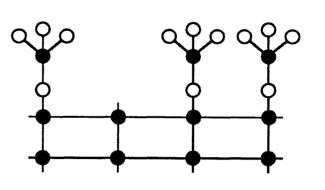
\includegraphics[width=0.4\textwidth]{images/ligacao_incompleta_silicio}}
\hfill
\subfloat[Interface com uma impureza,\label{figure:interface_impureza}]{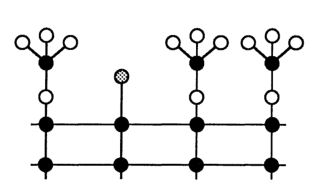
\includegraphics[width=0.4\textwidth]{images/interface_impureza}}
\hfill
\subfloat[Tipos de defeitos possíveis: ligação incompleta de silício e impureza no dióxido de silício\label{figure:tipos_impureza}]{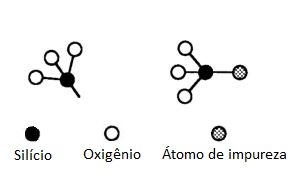
\includegraphics[width=0.4\textwidth]{images/tipos_impureza}}
\caption{Armadilhas para elétrons e lacunas em uma estrutura de $Si-SiO_2$ \cite{Leblebici1993}.}
\label{figure:modelos_armadilhas}
\end{figure}
\subsubsection{Hot Carrier Injection}
\label{subsection_HCI}
\textit{Hot Carrier Injection} (HCI) é um dos efeitos mais antigos e estudados, tendo sido introduzido por Shockley em 1961 para explicar fenômenos em junções \textit{p-n} à época \cite{Shockley1961}. O campo elétrico próximo à região de dreno de um transistor (e.g., \textit{MOSFET}) é considerado como a principal causa deste efeito, onde alguns portadores possuem uma energia cinética muito alta em comparação à média dos demais. Tais portadores de alta energia possuem uma temperatura efetiva acima da ambiente (``mais quentes'') e são capazes de vencer o potencial da superfície e são injetados no óxido de porta.

Parte destes portadores permanecem no óxido, gradualmente acumulando cargas e alterando a tensão de limiar $V_{TH}$ e a condutância $g_{o}$ ao longo da vida do dispositivo. Na década de 80 estes efeitos começaram a chamar a atenção, como consequência da redução contínua da escala dos transistores sem que existisse uma redução da tensão de alimentação \cite{Takeda1983}.

Já na década de 90, o \textit{HCI} foi mitigado com a redução da tensão de operação, redução esta que visava primeiramente um menor consumo de energia \cite{Maricau2013}. Entretanto, a variação da tensão não tem acompanhado a miniaturização \cite{Wang2007}\cite{Bravaix2009} dos dispositivos, não contribuindo significantemente com a redução desta degradação. Apesar de ser considerado menos relevante em dispositivos pMOS em comparação à dispositivos nMOS (pois as lacunas são mais pesadas que elétrons) o \textit{HCI} pode, ainda assim, realçar outros efeitos de envelhecimento \cite{Parthasarathy2006}. Atualmente quatro mecanismos de HCI são largamente conhecidos e estudados \cite{Maricau2013}:
\begin{enumerate}
\item \textbf{Channel Hot Electron (CHE):} Alguns elétrons ``sortudos'' (i.e., \textit{lucky electrons}), possuindo energia o suficiente, vencem a barreira da interface $Si/SiO_{2}$ na região do canal próxima ao dreno (ver figura \ref{figure:CHE_HCI}). Caso a tensão na porta $V_{g}$ seja baixa, o campo elétrico resultante não atrai suficientemente elétrons para a porta.   Quando a tensão  é aproximadamente igual à tensão do dreno $V_{d}$, atinge seu considerado valor máximo;
\item \textbf{Substrate Hot Electron (SHE):} Quando uma grande diferença de potencial é aplicada no corpo do transistor, seja positiva ou negativa, os portadores são direcionados para a interface $Si/SiO_{2}$ adquirindo energia cinética o suficiente para vencer a barreira ao longo de toda a interface do canal  e eventualmente sendo injetado no óxido de porta (ver figura \ref{figure:SHE_HCI}) uniformemente;
\item \textbf{Drain Avalanche Hot Carrier (DAHC):}  Em determinadas condições de estresse, onde a tensão $V_{d}$ no dreno é alta e a tensão $V_{g}$ é baixa, portadores de alta energia cinética podem colidir com elétrons, que antes estavam  ligados à estrutura cristalina, cedendo a eles energia, deixando-os livres para condução e criando um par elétron-lacuna no local \cite{Sze2007}. Estes, por sua vez, são acelerados mediante influência do campo elétrico no canal e podem potencialmente vencer a barreira da interface $Si/SiO_{2}$, ficando presos na região ou criando estados interfaciais (ver figura \ref{figure:DAHC_HCI}). Pode existir ainda uma componente adicional de corrente no corpo do transistor (i.e., \textit{bulk});
\item \textbf{Secondary Generated Hot Electron (SGHE):} esse efeito compreende a criação de portadores ``quentes'' (\textit{i.e.} hot carriers, HC) através da ionização por impacto envolvendo um segundo portador, sendo este também gerado por uma anterior ionização por impacto (e.g., \textit{DAHC}). Os primeiros portadores podem gerar durante seu deslocamento, por influência do campo transversal, novos portadores que, também acelerados por este campo em direção à interface, adquirem energia suficiente para a superar a barreira e atravessar o material (ver figura \ref{figure:SGHE_HCI}). Apesar disso, este efeito é considerado como um contribuinte inferior na degradação dos transistores se comparado aos demais efeitos \cite{Maricau2013}.
\end{enumerate}
\begin{figure}[H]
\center
\subfloat[CHE\label{figure:CHE_HCI}]{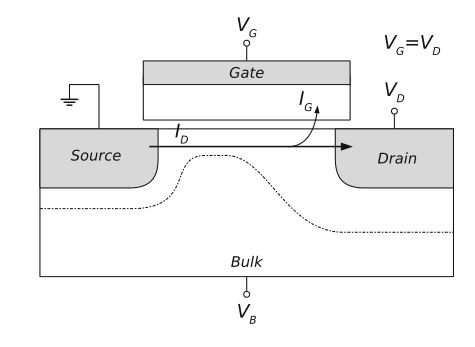
\includegraphics[width=0.45\textwidth]{images/CHE_HCI}}
\hfill
\subfloat[SHE\label{figure:SHE_HCI}]{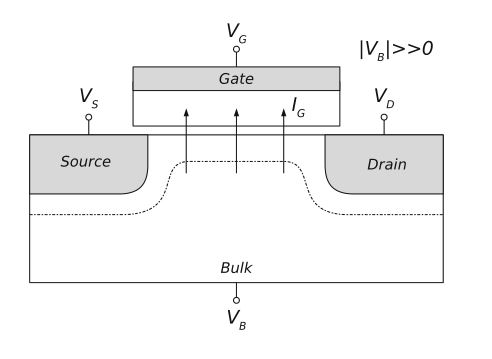
\includegraphics[width=0.45\textwidth]{images/SHE_HCI}}
\hfill
\subfloat[DAHC\label{figure:DAHC_HCI}]{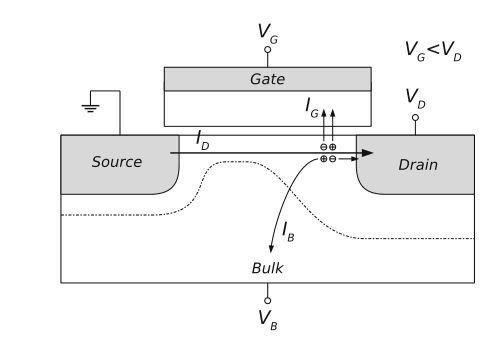
\includegraphics[width=0.45\textwidth]{images/DAHC_HCI}}
\hfill
\subfloat[SGHE\label{figure:SGHE_HCI}]{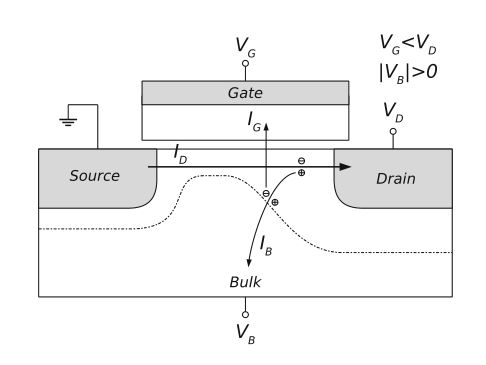
\includegraphics[width=0.45\textwidth]{images/SGHE_HCI}}
\caption{Mecanismos de injeção de portadores \cite{Maricau2013}.}
\label{figure:mecanismos_HCI}
\end{figure}
Estes quatro mecanismos se manifestam no transístor em diferentes condições de operação, sendo o DAHC e o CHE os que mais contribuem para a degradação do dispositivo. Para transistores de 0.35${\mu}$m, o DAHC é mais proeminente do que os demais efeitos. Já para dimensões inferiores, o CHE é considerado o efeito de degradação dominante \cite{Takeda1983}.
A variação na tensão de limiar através de HCI foi modelada como dependente do tempo, do campo elétrico no óxido $(E_{ox})$, do campo elétrico lateral máximo $(E_{lat})$, da temperatura $(T)$ e do comprimento do transistor $(L)$ :
\begin{equation} \label{eq:HCI1}
\Delta V_{TH} = A_{HCI}t^{n_{HCI}}
\end{equation}
sendo $A_{HCI}$ quantificado por \cite{Maricau2008}\cite{Kufluoglu}\cite{ChenmingHu1985}:
\begin{equation} \label{eq:HCI2}
A_{HCI} \propto \frac{1}{\sqrt{L}}exp \left(\alpha_{HCI,1}E_{ox}\right)exp\left(-\frac{\alpha_{HCI,2}}{E_{lat}}\right)
\end{equation}
onde $\alpha_{HCI,1}$ e $\alpha_{HCI,2}$ são parâmetros específicos da tecnologia.

\subsubsection{Bias Temperature Instability}
\label{subsection_BTI}
Conhecido de forma genérica por BTI (Bias Temperature Instability), é considerada uma das ameaças mais críticas em tecnologias CMOS. Apesar de conhecido há bastante tempo, este efeito tem se tornado mais proeminente em tecnologias abaixo de 90nm \cite{Amat2009}.

Este efeito é influenciado pela temperatura e se mostra presente quando uma tensão estressante é aplicada na porta do transistor, sendo percebido como uma alteração nos parâmetros de operação do transistor, tipicamente a tensão de limiar $V_{TH}$. No caso do NBTI, (\textit{i.e.} Negative BTI) esse fenômeno é observado em pFETs e em nFETs para o PBTI. Ainda n\~{a}o há um pleno consenso sobre a origem do BTI (a n\'{i}vel microsc\'{o}pico).

Alguns pesquisadores s\~{a}o de opini\~{a}o que este efeito surge de uma combinaç\~{a}o do aprisionamento de portadores nas imperfeiç\~{o}es do \'{o}xido e a geraç\~{a}o de estados na interface do canal do \'{o}xido.
Uma propriedade singular deste mecanismo se torna aparente em situaç\~{o}es nas quais s\~{a}o aplicadas tens\~{o}es estressantes sobre o dispositivo. Esta propriedade, conhecida como \textit{relaxamento} ou \textit{recuperaç\~{a}o}, indica a reduç\~{a}o da degradaç\~{a}o em um momento imediatamente posterior ao da apliaç\~{a}o da diferença de potencial estressante.

Por este motivo, a modelagem do BTI \'{e} complexa, com indícios de degradação residual após o relaxamento das condições de estresse, sendo indicados por duas componentes: uma permanente e outra recuperável \cite{Maricau2013}.
Alguns estudos modelam então este efeito como consequência de dois mecanismos \cite{Cho2010}:
\begin{enumerate}
\item
Geração de imperfeições próximas a interface entre silício e óxido, resultando numa componente de probabilidade de tunelamento dos átomos de Hidrogênio (H+);
\item E uma componente de recuperação, quantificando a captura e soltura de portadores.
\end{enumerate}
Este comportamento é matematicamente expresso da seguinte forma:
\begin{equation} \label{eq:BTI_permanent_recoverable}
\Delta V_{TH} \propto \left[ \underbrace{exp(\alpha_1 V_{GS})t^{n_P}}_{\text{Componente permanente}} + \underbrace{V_{GS}^{\alpha_2}(C_R + n_R \log_{10}({t}))}_{\text{Componente recuperável}} \right] exp\left(-\frac{E_a}{kT}\right)
\end{equation}

sendo a variação da tensão de limiar, $\Delta V_{TH}$, uma função do campo elétrico $(E_{ox})$ aplicado no óxido de porta do transistor e a temperatura $(T)$. Os parâmetros $\alpha_1$ e $\alpha_2$ são fatores de escalonamento da voltagem e dependentes da tecnologia empregada, $E_a$ é a energia de ativação correspondente, $C_R$, $n_P$ e $n_R$ são expoentes de ajuste do tempo para as componentes permanente e recuperável, e $k$ é a constante de Boltzman.

É importante salientar que a equação \ref{eq:BTI_permanent_recoverable} só é válida para uma voltagem estressante que seja invariante, sendo necessária um modelo mais preciso para o BTI quando a tensão aplicada é variante no tempo \cite{Grasser2009a}.
Os efeitos de BTI s\~{a}o considerados determin\'{i}sticos para transistores de tamanho microm\'{e}trico, com uma variaç\~{a}o id\^{e}ntica nos par\^{a}metros dos transistores \cite{Wang2007}.

Porém, ao serem reduzidos para a escala nanométrica, estes efeitos passam a ser considerados como estocásticos. A mudança dos parâmetros dos transistores varia com o tempo. Além disso, estas mudanças são intensificadas pelo aumento do desvio padrão deste mesmos parâmetros, também no tempo. 
\subsubsection{Time-Dependent Dieletric Breakdown}
\label{subsection_TDDB}
A operação adequada de um transistor MOS exige que o mesmo esteja operando sob as corretas condições, incluindo aí a magnitude do campo elétrico aplicado na sua região isolante. Estes campos elétricos podem eventualmente exceder o campo elétrico máximo suportado pelo dielétrico e levá-los à ruptura. Como consequência há um acréscimo substancial da corrente na porta deste transistor.

Mas mesmo durante a operação normal de transistores, diferentes estados de ruptura podem se manifestar, sendo importante diferenciar as categorias existentes e em quais condições elas podem surgir, quais sejam \cite{Maricau2013}:
\begin{enumerate}
\item \textbf{Soft breakdown (SBD)}: é observada como uma perda parcial das propriedades dielétricas, em comparação com o \textit{Hard Breakdown}, e que n\~{a}o impede a operaç\~{a}o do mesmo. Apesar disso, o dispositivo passa a operar em condiç\~{o}es n\~{a}o idealizadas pela sua especificaç\~{a}o. Entretanto possuem apenas um pequeno aumento da corrente de porta e a completa quebra do dispositivo é improvável \cite{Maricau2013};
\item \textbf{Progressive breakdown (PBD)}: É um passo gradativo que surge após o SBD, sendo percebido como um pequeno incremento na corrente de porta no decorrer do tempo. É presenciado em estruturas de óxido ultra-fino, tipicamente abaixo de 2.5nm de espessura;
\item \textbf{Hard breakdowns (HBD)}: é percebida como um aumento significativo da corrente de porta e uma redução da controlabilidade da tensão de porta do dispositivo. Este tipo de ruptura em qualquer transistor é considerada como sendo capaz de causar uma falha permanente no circuito.
\end{enumerate}
O TTDB é entendido como sendo este processo de danificação gradual no óxido graças a estes fortes campos elétricos.
Apesar da importância do TDDB para o estudo da confiabilidade de transistores, os modelos f\'{i}sicos a n\'{i}vel molecular existentes são, de certa forma, especulativos \cite{McPherson2012}, divindo-se em tr\^{e} categorias principais: \textit{a)} modelamento pelo campo el\'{e}trico; \textit{b)} modelamento pela corrente el\'{e}trica; \textit{c)} e modelamento pela combinação de ambos. Apesar de não existir um modelo largamente aceito, existem algumas características que são amplamente reconhecidas \cite{McPherson2012}:
\begin{enumerate}
\item TDDB é fortemente dependente do campo;
\item TDDB pode ser fortemente dependente da temperatura;
\item TDDB pode ser dependente da polaridade;
\item Alguns defeitos, armadilhas e ligações incompletas podem ser formadas durante o estresse causado por TDDB;
\item A geração de falhas leva a criação de um caminho condutivo de infiltração que, eventualmente, ocasiona a quebra do dispositivo;
\item O TDDB pode ser estatisticamente descrito por distribuições de Weibull;
\item Os parâmetros de aceleração de partículas no campo crescem diretamente proporcional à constante dielétrica $\kappa$.
\end{enumerate}
Assim sendo, o entendimento do mecanismo por detr\'{a}s da quebra do diel\'{e}trico é de vital importância. Os defeitos gerados durante o estresse são normalmente consideradas como neutros pois não há mudança significativa do diagrama de banda de energia para um disposotivo MOS. Al\'{e}m disso, acredita-se que estes defeitos devem estar relacionados a um processo de geração de defeitos a nível molecular \cite{McPherson2012}. Ainda mais: a geraç\~{a}o de defeitos no material \'{e} considerada irrevers\'{i}vel.

Mesmo ap\'{o}s o recozimento do dispositivo ou a invers\~{a}o do campo, n\~{a}o há evid\^{e}ncia de um aumento significativo do tempo de vida. O entendimento passa a ser de que o dano causado permanece na rede de silício e é praticamente irreversível. Este tipo de comportamento é então associado à mudanças na ligação dos átomos. Durante a ruptura da ligação covalente do íon de silício, por influência do campo elétrico local, há a criação de ligações incompletas (\textit{i.e.} dangling bonds) que possuem apenas um elétron e de uma estrutura diferente (ver figura \ref{figure:mecanismos_TDDB_vacancies}).
\begin{figure}[H]
\center
\subfloat[Orientação tetraédrica da ligação Si-Si.\label{figure:TDDB_SiSi_tetra}]{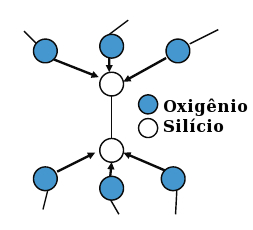
\includegraphics[width=0.45\textwidth]{images/TDDB_vacancies_a}
}
\hfill
\subfloat[A estrutura da rede é alterada após a quebra da ligação Si-Si e sofre forte influência de um campo $E_{loc}$ local àquela ligação incompleta. \label{figure:TDDB_SiSi_tri}]{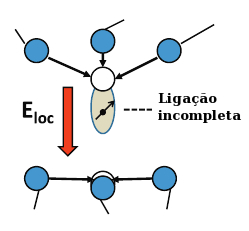
\includegraphics[width=0.45\textwidth]{images/TDDB_vacancies_b}
}
\caption{Geração de ligações incompletas a partir de vacâncias \cite{McPherson2012}.}
\label{figure:mecanismos_TDDB_vacancies}
\end{figure}
Esta estrutura pode ser ``relaxada'' a tal ponto que mesmo após o recozimento ou alteração do sentido do campo, como mencionado anteriormente, a ligação não será reparada, sendo esta uma das observações mais significantes do estresse provocado pelo TDDB.

Diversos modelos têm sido propostos para as categoria anteriormente mencionadas. Para o \textit{HDB}, os mais conhecidos são: modelo termoquímico (\textit{i.e.} termochemical), modelo injeção-anodo-lacuna (\textit{i.e.} anode-hole-injection) e o modelo direcionado à voltagem (\textit{i.e.} voltage-driven).
O modelo termoquímico é conhecido como \textit{modelo} $E$ (\textit{i.e.} E model), pois considera que existe uma correlação direta entre o campo elétrico aplicado no óxido do dispositivo $E_{ox}$ e o tempo de vida do dispositivo; sendo as ligações químicas no óxido fracas o suficiente para que este campo elétrico as rompa.

Assim sendo, o tempo para quebra (\textit{i.e.} time to breakdown) $t_{BD}$ é expresso por \cite{McPherson1985}:
\begin{equation} \label{eq:TDDB_time_to_break_Emodel}
t_{BD}\propto \exp\left(-\gamma E_{ox}\right)\exp\left(\frac{E_{a}}{kT} \right)
\end{equation}
onde $\gamma$ ($\gamma\approx$ 1.1década/MV/cm) é um fator de aceleração do campo e $E_a$ ($E_a\approx 0.6 - 0.9$eV) é a energia de ativação térmica.

Já o modelo injeção-anodo-lacuna é conhecido como \textit{modelo} $1/E$ e prevê uma dependência entre o $t_{DB}$ e o campo elétrico, sendo uma consequência da captura de lacunas em determinadas regiões do óxido de porta. Ela é expressa por \cite{ChenmingHu1985}:

\begin{equation} \label{eq:TDDB_time_to_break_1/Emodel}
t_{BD}\propto \exp\left(\frac{\beta}{E_{ox}}\right)\exp\left(\frac{E_{a}}{kT} \right)
\end{equation}
onde $\beta$ ($\beta\approx$ 350MV/cm) é um fator de aceleração do campo dependente do processo de fabricação.
Existem ainda modelos que combinam os dois propostos acima. De todo caso, estes modelos vem sendo revisados para óxidos de porta inferiores à 5nm \cite{Maricau2013}.
Na seção \ref{subsubsection_Modelos_TDDB} serão apresentados modelos mais precisos e modernos.

\subsection{Estado da arte}
\label{subsection_estado_da_arte}
As diversas técnicas de confiabilidade de circuitos integrados utilizadas para reduzir o impacto do envelhecimento se concentram em contramedidas tais como: blindagem de circuitos, faixas de segurança (\textit{i.e.} guard-banding), balanceamento de cargas, voltagem dinâmica e escalonamento de frequência \cite{Mintarno2010}\cite{Mitra2011}, se encaixando em uma outra das categorias definidas na seção \ref{subsubsection_tecnicas_hardware}.

Para suportar algumas destas estratégias deve-se prever a falha de um sistema com antecedência, usando tal informação para ajudar na tomada de decisões destas contramedidas antes mesmo que qualquer erro se manifeste. Esta estratégia se diferencia da abordagem clássica, que atua somente após o surgimento de erros. Uma abordagem que vêm sendo explorada é a de utilização de sensores variados em diversos locais do sistema, coletando informações sobre diversos parâmetros de operação ao longo do tempo. 

Eles podem ser analisados internamente ou externamente na procura de anomalias que indiquem que o sistema irá falhar. A frequência desta coleta pode ser ajustada a nível de design ou ser adaptativa durante a operação, permitindo que esta frequência seja adequada ao longo da operação para melhor capturar comportamentos que sejam anômalos ou que levem a uma degradação do sistema \cite{Agarwal2007}. Exemplos de dados a serem coletados são: temperatura, tensão de alimentação, atrasos, grau de atividades e outros que o projetista julgar importante.

Estes sensores podem ser \textit{in-situ}, adicionados a caminhos críticos específicos para detectar o não cumprimento de restrições de tempo; \textit{online self-testing}, onde um sistema entra em modo de teste e executa rotinas de \textit{Built-On Self Test} (BIST) que auxiliam na determinação da degradação corrente; \textit{sensores de envelhecimento}, que utilizam circuitos de referência espalhados pelo sistema que informam alteração em parâmetros de operação; e \textit{monitores de estresse}, que coletam informações de temperatura, alimentação e carga do sistema.

Técnicas como \textit{shadow transistors} incluem transistores paralelos entre aqueles que, previamente identificados, são considerados mais vulneráveis. Desta forma, não apenas o tempo de vida é melhorado como também são compensadas as falhas inseridas durante a fase de fabricação (\textit{e.g. circuitos abertos}). Esta medida não reduz a taxa de falha $\lambda$ de um determinado transistor mas inclui um caminho adicional em sua \textit{netlist}, reduzindo a probabilidade de falha, já que ambos os caminhos, tanto o original como a duplicata, devem falhar para que haja o sistema falhe \cite{Cornelius2008}.

Esta técnica pode ser realizada através da inserção guiada ou aleatória de \textit{shadow transistors}, conduzindo a resultados promissores. A técnica pode ser combinada com transistores de espessuras de óxido diferentes, aumentando ainda mais a confiabilidade de um sistema. Entretanto, tais técnicas têm como consequência o aumento da área, acréscimo do consumo dinâmico e do atraso médios.

Outra forma de aumentar a confiabilidade de um sistema é através da utilização de \textit{sleep transistors}. Estes transistores de alta tensão de limiar $V_{TH}$, sejam pMOS ou nMOS, são utilizados para interromper a alimentação de partes do sistema que eventualmente esteja em modo de espera. Entretanto, esta técnica necessita considerar diversos aspectos, tais como: ativação por nMOS ou pMOS, qual será a distribuição espacial dos \textit{sleep transistors}, largura e profundidade da porta, otimização área ocupada pelo corpo do transistor, fugas e eficiência \cite{Shi}.

Esses, por sua vez, podem ser utilizados para alternar a ativação de módulos do sistema. Ao desconectar a alimentação de um módulo ele não irá, idealmente, apresentar tensões ou correntes e consequentemente nenhum campo elétrico. A consequência é uma redução da temperatura e ausência de atividade. Isto é importante na redução de efeitos indesejados, tais como: eletromigração \cite{Srinivasan2003}, ruptura do óxido de porta e NBTI.

Então, durante a fase ociosa das portas este efeitos serão eliminados ou reduzidos drasticamente. Como consequência desejada, o MTTF é prolongado \cite{Torres2013}. Esta técnica é conhecida como \textit{Alternating Module Activation} (AMA).

Em abordagens mais recentes, a melhoria da confiabilidade de um sistema está sendo obtida através da adoção de técnicas de aprendizado de máquina (\textit{i.e.} machine learning) que permitem representar e prever qual é a degradação que um sistema sofre através da observação de caminhos críticos. Ao observar por um período de tempo $t$ qual é o acréscimo no atraso das saídas destes caminhos, estas informações são relacionadas à carga de trabalho a qual o sistema está submetido. Esta carga e este tempo $t$ são determinados durante o design e a predição é \textit{online}.

Tais informações de design (tempo de observação, caminhos críticos e saídas observáveis) são decididas pelo projetista e alteram a precisão da predição \textit{online}. Porém, durante a operação, as informações utilizadas pelo modelo podem ser atualizadas à conveniência do projetista. Esta decisão impacta a área ocupada pelo sistema, pois acarretará na inclusão de dispositivos à estrutura, tornando-a maior. Parte desta tarefa de monitoramento e predição pode ser dividida entre componentes de hardware e software, mitigando uma porção deste acréscimo de área e permitindo a integração de modelos mais complexos.

Trabalhos realizados nesta área relatam que esta estratégia apresenta uma boa precisão e é considerada promissora \cite{Baranowski2015}. Entretanto, estes trabalhos consideram somente alguns dos fenômenos de envelhecimento, tais como NBTI, e apenas parte das condições ambientais que contribuem para o envelhecimento de transistores (\textit{e.g.} temperatura, tensão de alimentação e atividade).

Essas diversas abordagens endereçam o mesmo problema mas sugerem ações diferentes, porém complementares. Isto é importante pois permite que tecnologias mais robustas de verificação, avaliação e relatórios se tornem viáveis. Ao atuarem em diversas camadas de abstração, que têm se tornado cada vez mais complexas, novas tecnologias podem integrar essas soluções, mitigando ou corrigindo erros e falhas nessas diferentes camadas. Assim sendo, a confiabilidade de um sistema é melhorada como um todo.

Em \cite{Maeda2014} temos um exemplo da empregabilidade de tais abordagens em uma tecnologia que, sendo uma proposta universal, integra e arbitra a comunicação entre estes elementos. 

\subsection{Modelos Compactos}
\label{subsection_modelos_compactos}

Na seção \ref{subsection_Conf_CI} foram apresentados os principais efeitos físicos responsáveis pelo envelhecimento de circuitos integrados. Foram apresentados ainda alguns modelos que se propõem a explicar as relações entre os parâmetros de operação e as degradações observadas. Esta seção discute o desenvolvimento de modelos compactos para transistores MOS.

Será discutido primeiramente os modelos existentes para HCI e em seguida para um enfoque nos modelos existentes para baias temperature instability e TDDB.
	
\subsubsection{Modelos para HCI}
\label{subsubsection_Modelos_HCI}

Considerado no início como um efeito de grande importância para explicar a degradação de transistores, o HCI se tornou um efeito menos dominante à medida que a tensão de alimentação foi sendo reduzida. Entretanto ele ainda é considerado um problema para tecnologias atuais visto que o campo elétrico vem aumentando gradativamente com a redução do tamanho dos transistores.

Diversos modelos foram publicados ao longo dos anos para explicar o HCI.  Entre eles o modelo do elétron ``sortudo'' (\textit{i.e. lucky electron model}, LEM) é um dos mais conhecidos. Além disso, muito dos outros modelos que surgem posteriormente são derivados do LEM. Em 1985 \cite{ChenmingHu1985} foi um dos primeiros a introduzir o modelo baseado no LEM. As propostas que se seguem utilizam a mesmo teoria mas propõem uma formulação analítica diferente ou propõem uma acomodação do modelo para tecnologias CMOS mais avançadas.

No trabalho apresentado em \cite{Kufluoglu} os efeitos de HCI e NBTI foram unificados em um mesmo modelo, levando em consideração a geração de armadilhas interfaciais devido a desassociação das ligações de Si-H. Posteriormente esta proposta é utilizada para desenvolver outros modelos para tecnologias mais avançadas. Um modelo semi-empírico foi proposto e pode ser expressado de acordo com a quantidade de estados interfaciais gerados:
\begin{equation}\label{eq:HCI_semi_empircal_states}
\Delta N_{IT}=C_1\left[\frac{I_{DS}}{W}\exp\left(-\frac{\phi_{IT,e}}{q\lambda_eE_{lat}}\right)T_{str}\right]^n
\end{equation}
onde $W$ é a largura de canal do transistor, $I_{DS}$ é corrente dreno-fonte, $E_{lat}$ é o campo elétrico lateral máximo no dreno, $T_{str}$ é o tempo de estresse ao qual o transistor é submetido, $\phi_{IT,e}$ é a energia crítica necessária para que os elétrons criem uma armadilha interfacial \cite{Maricau2013}. 

Apesar desses modelos serão baseados no LEM, eles incluíam apenas uma fonte de portadores ``quentes''. Entretanto, como mostrado anteriormente na seção \ref{subsection_HCI}, existem outros três mecanismos que foram identificados ao longo dos anos de pesquisa e que podem potencialmente resultar em uma mudança no comportamento do transistor ao longo do tempo.

Posteriormente, \cite{Maricau2013} propôs um modelo baseado em uma abordagem conhecida como reação-difusão (\textit{i.e. reaction-diffusion}, RD) proposta em \cite{Kufluoglu} e também baseado no LEM. O modelo RD possui alguns pontos negativos ao tentar modelar o BTI. Um desses é a incapacidade de considerar o aprisionamento de óxidos.

Entretanto esse efeito está relacionado ao fenômeno de recuperação do BTI, que ocorre após o estresse aplicado no dispositivo cessar. Entretanto, esse modelo ainda pode ser utilizado para modelar o efeito de HC, visto que as armadilhas interfaciais são geradas próximas ao fim da região do dreno, onde efeito de recuperação é negligenciável.

É utilizado então um conjunto de duas equações diferenciais que descrevem a geração das partículas de hidrogênio próximas à interface óxido canal e qual é a sua difusão em direção ao contato da porta. Essas equações são então resolvidas numericamente ao sinalizar um transistor. Porém essa análise não é apropriada para o estudo de um circuito inteiro.

Em \cite{Maricau2013}, é proposta uma expansão deste modelo, válido somente para tensões de estresse contínuas (modelo DC). Entretanto circuitos integrados atuais são submetidos a tensões que variam no tempo. Para incluir essa variação uma extensão ao modelo DC deve ser incluída, um modelo AC. 

Ainda em \cite{Maricau2013}, ambos os modelos, AC e DC, são combinados para avaliar o impacto do HCI no comportamento do transistor graças à sinais estressantes variantes no tempo.

\subsubsection{Modelos para BTI}
\label{subsubsection_Modelos_BTI}

Para  transistores cuja tecnologia está abaixo de 90 nanômetros, o NBTI é considerado uma das maiores ameaças a confiabilidade de dispositivos. Assim sendo, é considerado essencial prever quais são os impactos desse efeito na performance de circuitos integrados. Apesar de também presente, o PBTI recebe um enfoque menor.

Um dos principais desafios enfrentados ao se analisar este efeito é explicar o comportamento dele a nível microscópico. Na década de 70, algumas pesquisas já sugeriam que a criação de estados na interface estava relacionada ao mecanismo de difusão do hidrogênio. Esse mecanismo foi posteriormente chamado de reação-difusão (RD). Em 2006 foi sugerido que o NBTI consiste de uma geração de estados na interface mais ou menos constante combinada a um componente de recuperação relacionada ao aprisionamento de lacunas \cite{Parthasarathy2006}.
\\

\textbf{Modelo de Reação-Difusão}

Este modelo propõe que uma reação ativada termicamente entre lacunas e ligações de Si-H na interface dielétrico/substrato do MOSFET resulta na geração de ligações incompletas. Estas por sua vez levam ao surgimento de estados interfacias. As partículas de hidrogênio se afastam da interface por difusão e vão em direção ao dielétrico de porta.

O modelo mais conhecido foi proposto em \cite{Alam2003} e posteriormente aperfeiçoado por outras pesquisas \cite{Schroder2003}\cite{Chakravarthi2004}. De acordo com o modelo RD. Esta reação eletroquímica é então definida como depende da temperatura e do campo; e a taxa da geração de armadilhas é descrita pela seguinte equação diferencial:
\begin{equation}\label{eq:BTI_RD_diff}
\frac{d N_{IT}}{dt} = k_F\left(N_0 - N_{IT}\right) - k_RN_H(0)N_{IT}
\end{equation}
sendo $N_{IT}$ uma variável para representar a quantidade de armadilhas interfaciais, $N_0$ é a quantidade inicial de ligações incompletas de Si-H e $k_F$ é uma constante que representa a taxa de desassociação depende do campo no óxido. $k_R$ é a taxa de recozimento das ligações incompletas associada aos átomos de hidrogênio. $N_H(0)$ é a concentração de hidrogênio na interface. Entretanto, os átomos de hidrogênio podem difundir da interface para dentro do óxido, sendo este processo descrito por:
\begin{equation}\label{eq:BTI_RD_hydrogen_diff}
\frac{d N_{H}}{dt} = D_H\frac{d^2N_H}{dx^2}
\end{equation}
onde $N_H$ é a concentração total de hidrogênio no óxido e $D_H$ é uma constante de difusão. Estas ligações incompletas atuam como armadilhas ``doadoras'' que contribuem para variação na tensão de limiar $V_{TH}$, que pode ser representada por:
\begin{equation}
\Delta V_{TH}=\frac{qN_{IT}}{C_{ok}}
\end{equation}
sendo $q$ a carga de um elétron e $C_{ox}$ a capacitância do óxido de porta.

A figura \ref{figure:RD_model} mostra de forma simplificada onde estes fenômenos ocorrem.
\begin{figure}
\center
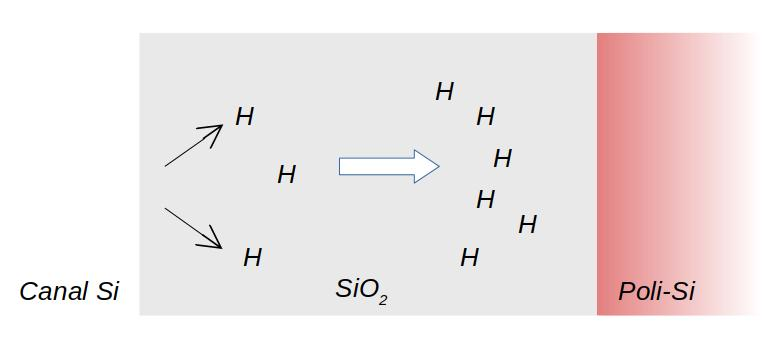
\includegraphics[width=0.5\textwidth]{images/RD_model}
\caption{Representação da quebra de ligações Si-H e Si-O na interface $Si/SiO_2$}
\label{figure:RD_model}
\end{figure}
\subsubsection{TDDB}
\label{subsubsection_Modelos_TDDB}

Como explicado anteriormente na seção \ref{subsection_TDDB}, a quebra do óxido de porta pode se dar em etapas, indo de um Soft Breakdown (SBD) a um Hard Breakdown (HBD); sendo necessário então descrever quais mecanismos estão envolvidos nestas duas etapas e como podemos modelar tal comportamento.
\\

\textbf{Modelo para Hard Breakdown}

Existem diversos modelos que se propõe a explicar este fenômeno, sendo um dos mais conhecidos o modelo \textit{termoquímico}. Entretanto ele foi gradativamente modificado para atender a resultados obtidos em experimentos posteriores, que indicavam que as formulações descritas nas equações \ref{eq:TDDB_time_to_break_Emodel} e \ref{eq:TDDB_time_to_break_1/Emodel} não eram mais válidas para óxidos de porta com espessuras menores do que 5nm \cite{Wu2001}.

O modelo foi expandido posteriormente para incluir a dependência da área e a distribuição do \textit{tempo para ruptura} \cite{Wu2005}, visto que anteriormente só era prevista o tempo para quebra característico. Entretanto, alguns dispositivos falhavam antes desse tempo.

Considerando estas mudanças, um modelo completo para tempo de quebra em óxidos ultrafinos (\textit{i.e.} $t_{ok} < 5nm$) pode ser descrito por:
\begin{equation}\label{eq:TDDB_complete_model}
t_{BD}\propto \left(\frac{1}{WL}\right)^{1/ \beta}F_{BD}^{1/\beta}V_{GS}^{a+bT}\exp\left(\frac{c}{T} + \frac{d}{T^2}\right)
\end{equation}
sendo $W$ e $L$ a largura e o tamanho do transistor, respectivamente. As contantes $\beta$, $a$, $b$, $c$ e $d$ são dependentes da dimensão do transistor CMOS \cite{Li2008}.

O tempo de quebra segue uma distribuição de Weibull e sua função de probabilidade de falha cumulativa $F_{BD}$ é descrita por:
\begin{equation}\label{eq:TDDB_probability_function}
F_{BD}=1-\exp \left(-\frac{t}{t_{BD,63}}\right)^\beta
\end{equation}

\textbf{Modelo para Soft Breakdown}

Passando a ser importante com o advento de dielétricos ultrafinos, o SBD não se traduz na perda de controlabilidade da tensão de porta do transistor mas sim em um pequeno acréscimo da corrente de porta e na criação de um caminho de infiltração no óxido. Porém, assim como o HBD, o SBD também segue uma distribuição de Weibull.

Essa infiltração no óxido é gradual e em concordância com o pequeno incremento da corrente de porta encontrado experimentalmente \cite{Sahhaf2009}. Isso significa também que um único ponto de infiltração tem uma baixíssima probabilidade de impedir o funcionamento de um circuito. Porém um conjunto deles ao longo do tempo aumenta essa chance, sendo necessário modelar a quantidade de pontos de infiltração após um período de estresse.

A probabilidade de existirem $n$ defeitos de SBD em um instante de tempo $\chi$ pode ser descrita por uma distribuição de Poisson \cite{Wu2005}:
\begin{equation}
P_n(t)=\frac{\chi^n}{n!}\exp(-\chi)
\end{equation}
\begin{equation}
\chi = \left(\frac{t}{t_SBD,63} \right)^\beta
\end{equation}
\begin{equation}
t_{SBD,63} = t_{SBD,ref} \left(\frac{WL}{A_{ref}}\right)^{1/\beta}\left(\frac{V_{GS}}{V_{ref}}\right)^\gamma
\end{equation}
onde $t_{SBD,63}$ está associado ao tempo de quebra no 63º percentil para um transistor de referência de área $A_{ref}$ estressado a uma tensão $V_{ref}$. $\beta$ e $\gamma$ são parâmetros dependentes do processo do transistor \cite{Sahhaf2009}.

Este modelo entretanto não é dinâmico, pois não considera mudanças na tensão de estresse aplicada, mudanças estas que são consequência da alteração dos parâmetros de operação do transistor; e esta alteração é induzida justamente pelo envelhecimento.

Em \cite{Maricau2013} o modelo é alterado para considerar este dinamismo e descrever a probabilidade $P_n(t_2)$ de encontrar $n$ pontos de SBD em um instante de tempo $t_2$. Ela está relacionada à probabilidade $P_n'(t_1)$ de encontrar n' pontos de SBD no instante de tempo $t_1$:
\begin{equation}
P_n(t_2)=\sum_{n'=0}^{\infty}\left[P_{n'}(t_1)\frac{\Delta \chi^{n-n'}}{(n-n')!}\exp(-\Delta\chi) \right]
\end{equation}
\begin{equation}
\Delta\chi = \left(\frac{t_2-t_1}{t_{SBD|V_{GS1}=V{GS2}}} \right)^\beta
\end{equation}
sendo $V_{GS1}$ a tensão de estresse em $t_1$ e $V_{GS2}$ em $t_2$.
\subsection{Simuladores}
\label{subsection_Simuladores}

Com os efeitos de envelhecimento de transistores possuindo um impacto cada vez maior, a simulação da confiabilidade de circuitos eletrônicos se tornou uma parte importante em um fluxo moderno de design. Simulações precisas da confiabilidade permitem que o projetista aumente significantemente o design, satisfaça especificações mais complexas e ainda assim garanta uma operação confiável do sistema.

Diversas ferramentas surgiram na década de 70 após o advento do simulador \textit{SPICE}. Apartir daí, a complexidade das ferramentas seguiu o avanço dos métodos utilizados para caracterizar o envelhecimento de transistores e são construídos ao redor do \textit{SPICE} \cite{Maricau2013}.

Este trabalho utiliza o simulador Relxpert$^{\copyright}$ (Cadence Systems$^{\copyright}$), baseado no \textit{BERT\copyright}, que fornece um modelo analítico descrevendo cada efeito de envelhecimento. Normalmente, os modelos devem ser fornecidos pelos fabricantes, mas podem ser desenvolvidos pelo próprio pesquisador. Esses modelos devem descrever as mudanças nos parâmetros dos dispositivos como função da idade do transistor. Apesar de utilizar esta ferramenta, a metodologia que será apresentada independente da escolha feita pelo pesquisador.

